\chapter{Method}
\label{ch:3}
\label{sec:3}


\section{Overview}
\label{sec:3_1}


\subsection{Pipeline Architecture}
\label{sec:3_1_1}


The pipeline developed in this study is designed to examine how replacing measured or administrative building attributes with attributes inferred from street-view imagery, and subsequently converting those inferred attributes into U-values through a fixed TABULA/archetype lookup, affects downstream EPC classification and physical consistency. Data processing comprises four sequential stages. First, street-view images are paired with the target buildings, while the image source, view quality, and pairing status are retained. Second, eligible images are used to infer building type, construction year, and floor-related attributes, with the predicted values and unreadable cases recorded separately. Third, only the attributes required by the lookup key are used to deterministically assign each building to a TABULA/archetype cell, from which the substituted thermal parameters and their provenance are obtained. Fourth, the features required by the downstream model are assembled for each experimental route, and the physical parameters required to calculate \(H'_{\mathrm{tr}}\) are prepared.


The evaluation design is defined separately from the preceding data-processing stages. M1 uses reference attributes or reference thermal parameters, whereas M3 replaces the corresponding inputs with attributes inferred from street-view imagery and the results of the associated archetype lookup; together, these routes form the primary substitution comparison. M2 instead predicts EPC directly from imagery and serves as a parallel end-to-end comparator rather than an intermediate stage of the archetype pipeline. All comparable routes use the same geographic split. Binary EPC classification is the primary task, while seven-class EPC prediction is used to diagnose the information ceiling associated with fine-grained labels. LOCO evaluates cross-location generalisation, and \(H'_{\mathrm{tr}}\) provides a physical consistency check for the substituted thermal parameters.


\begin{figure}[htbp]
\centering
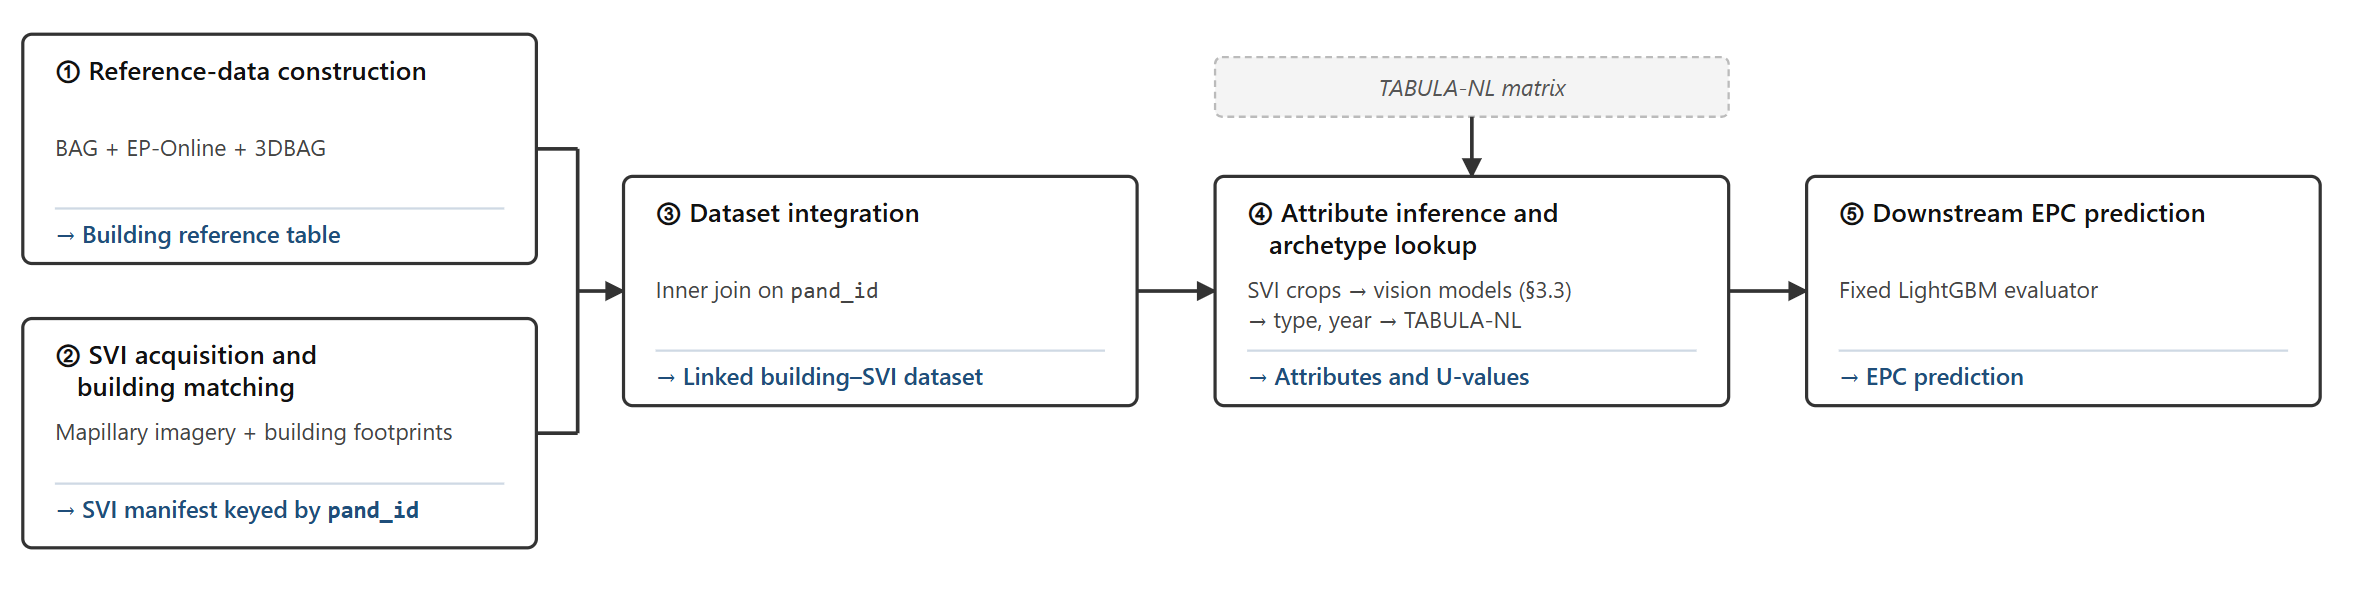
\includegraphics[width=0.98\linewidth,height=0.78\textheight,keepaspectratio]{figures/fig/fig_3_1_workflow.png}
\caption{End-to-end study workflow.}
\label{fig:3_1}
\end{figure}


\subsection{Semi-Synthetic Dataset: Three-Layer Structure}
\label{sec:3_1_2}


This study defines the semi-synthetic dataset as three layers with explicitly separated provenance. First, the reference layer contains administrative records from BAG and EP-Online, reconstructed geometry from 3DBAG, and the EPC reference label adopted in this study. These fields provide the reference observations required for model training, attribute substitution, and downstream evaluation, but they are not collectively treated as error-free ground truth. In particular, the EPC reference label remains affected by multiple certificates and within-building label disagreement; its quality is audited separately in \cref{sec:4_3_4}.


Second, the vision-inference layer stores the building-level predictions of building type, construction year, and floor count produced by the three vision paradigms, together with their model provenance. Third, the synthetic archetype layer derives the construction period from the estimated year, deterministically maps the pair (type, period) to a TABULA-NL cell, and assigns the cell's four as-built envelope U-values for the wall, roof, floor, and windows. These U-values are archetype-level average assumptions for the corresponding building-stock subgroup; they are not measurements of the thermal performance of individual buildings and do not introduce new building-specific observations.


Here, semi-synthetic refers to the combination of reference observations, image-derived attributes, and deterministically assigned archetype parameters. The EPC target remains an administrative reference label obtained from EP-Online rather than a simulated energy label; only the archetype parameters assigned through the TABULA cell are synthetic. This separation makes the provenance of each value traceable and provides the common data foundation for the three research objectives.


In the controlled substitution comparison, M1 and M3 use the same eligible buildings, geographic split, feature positions, and fixed model for each downstream task. M1 uses the reference type, year, and floor attributes and obtains the TABULA U-values from the corresponding reference (type, period) cell. M3 replaces these inputs with the type, year, and floor attributes inferred from SVI and retrieves the U-values from the resulting predicted cell. Within this protocol, the difference between M3 and M1 therefore measures the consequence of substituting the attribute source rather than the effect of retraining the downstream model. M2 predicts EPC directly from imagery and does not pass through this three-layer substitution chain; it is consequently treated as a parallel end-to-end comparator.


\begin{figure}[htbp]
\centering
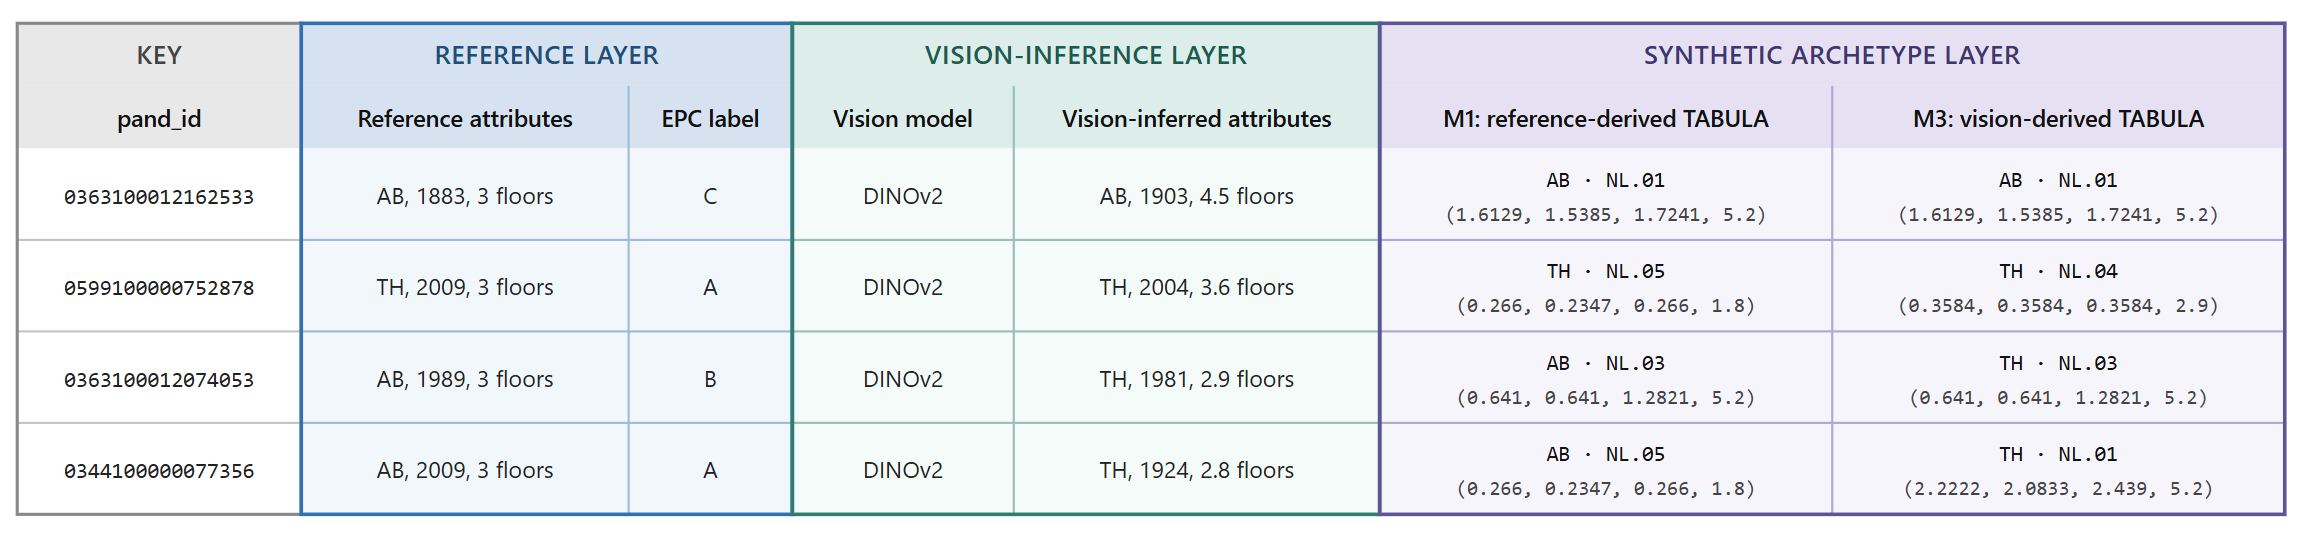
\includegraphics[width=0.98\linewidth,height=0.78\textheight,keepaspectratio]{figures/fig/fig_3_2_layers.png}
\caption{Three-layer semi-synthetic dataset structure.}
\label{fig:3_2}
\end{figure}


\section{Dataset Construction}
\label{sec:3_2}


\subsection{Sources}
\label{sec:3_2_1}


The dataset is constructed around the BAG \texttt{pand\_id} as the building-level identifier and integrates five public or openly licensed data sources: BAG, 3DBAG, EP-Online, Mapillary, and TABULA-NL. The building-level linkage of BAG, EP-Online, and Mapillary forms the core sample; 3DBAG provides the reconstructed geometry used in subsequent stages, while TABULA-NL provides a deterministic archetype lookup based on building type and construction period. The position of each source within the three-layer data structure is shown in \cref{fig:3_2}, and the principal fields and their roles in the study are summarised in \cref{tab:3_1}.



\begin{table}[H]
\centering
\caption{Data sources, principal fields, and roles in the study}
\label{tab:3_1}
\small
\begin{tblr}{
  width = \linewidth,
  colspec = {X[1,l] X[1,l] X[1,l]},
  row{1} = {font=\bfseries},
  rowsep = 3pt,
  colsep = 4pt
}
\toprule
Source & Main contents & Role in this study \\
\midrule
\textbf{BAG} & \texttt{pand\_id}, \texttt{bouwjaar}, two-dimensional building footprints, and building status & Building-level join key, construction-year reference, and residential-stock filtering \\
\textbf{3DBAG} & LoD2.2 reconstructions of floor count, height, volume, and envelope areas & Floor-count reference, Tier B reconstructed geometry, and area inputs for \(H'_{\mathrm{tr}}\) \\
\textbf{EP-Online} & \texttt{Energieklasse}, \texttt{Gebouwtype}, and \texttt{Registratiedatum} & EPC reference label, building-type reference, and certificate selection by date \\
\textbf{Mapillary} & Crowdsourced street-view imagery and image metadata & Vision-model input, SVI--building pairing, and image provenance \\
\textbf{TABULA-NL} & Six construction periods \ensuremath{\times} four size classes, comprising 24 archetype cells & Deterministic lookup from (type, period), providing as-built U-values for walls, roofs, floors, and windows \\
\bottomrule
\end{tblr}
\end{table}


Mapillary was selected instead of a commercial street-view service because its open licensing supports a reproducible research workflow. However, its image coverage is determined by contributor activity and does not constitute a random sample of the building stock. The resulting dataset may therefore be biased towards image-dense urban centres and particular residential types. Representative cropped street-view images are shown in \cref{fig:3_4}; the coverage bias is quantified through the sample distributions in \cref{sec:4_1_1}, and its implications for the scope of the study are discussed in \cref{sec:5_2}.


The downstream labels are constructed directly from the EP-Online \texttt{Energieklasse}, with ratings from A+ to A++++ first merged into class A. The primary task is an independently trained binary EPC classification task that groups the labels into A--C and D--G; the division between the two groups corresponds to the upper boundary of EPC class C at 250 kWh/(m\textsuperscript{2}·yr). Seven-class A--G prediction is retained as a diagnostic task for examining the information ceiling associated with fine-grained labels. Both tasks are derived directly from the registered \texttt{Energieklasse}; continuous-energy regression is an auxiliary analysis and is not used to define the primary labels.


\subsection{SVI Acquisition, Data Linkage, and Screening Rules}
\label{sec:3_2_2}


\textbf{SVI acquisition and image--building pairing.} This study uses a locally adapted version of the OpenFACADES framework \hyperlink{ref:liang2025}{(Liang et al., 2025)} to acquire and process Mapillary street-view imagery; the complete workflow is shown in \cref{fig:3_3}. OpenFACADES first acquires and integrates building footprints from OpenStreetMap and Overture Maps. In this study, the workflow is divided into separate footprint-acquisition and image-processing stages, with BAG-based residential pre-filtering introduced between them so that footprints outside the target residential stock do not enter the subsequent image-processing workflow.


Residential pre-filtering is performed using the geometric centroid of each footprint. The OpenFACADES footprints and BAG building polygons are first transformed to the Dutch national coordinate reference system EPSG:28992, after which the geometric centroid of each OpenFACADES footprint is calculated. A footprint is retained only when its centroid falls within a BAG residential-building polygon. This preliminary step determines only which footprints proceed to image processing.


For the retained footprints, OpenFACADES acquires metadata for Mapillary 360\ensuremath{^\circ} panoramic images within the study area and performs isovist analysis using a 30 m search radius to establish candidate pairings between panoramic images and visible buildings. Following angle-of-view (AoV) screening, the candidate images are downloaded at a resolution of 2,048 pixels. GroundingDINO is then used to detect the target building, and perspective reprojection and cropping are applied to produce single-building images before the final image-quality filtering stage.


Each cropped image retains its OpenFACADES \texttt{building\_id}, whereas the building attributes and energy labels in this study use the BAG \texttt{pand\_id} as their primary key. After image processing, the same centroid-based matching rule is therefore applied to create the formal crosswalk between the OpenFACADES \texttt{building\_id} and BAG \texttt{pand\_id}. When the centroid of a footprint falls within a BAG residential-building polygon, the building's \texttt{pand\_id} is assigned to the corresponding images. Images for which no BAG match can be established are excluded.


\begin{figure}[htbp]
\centering
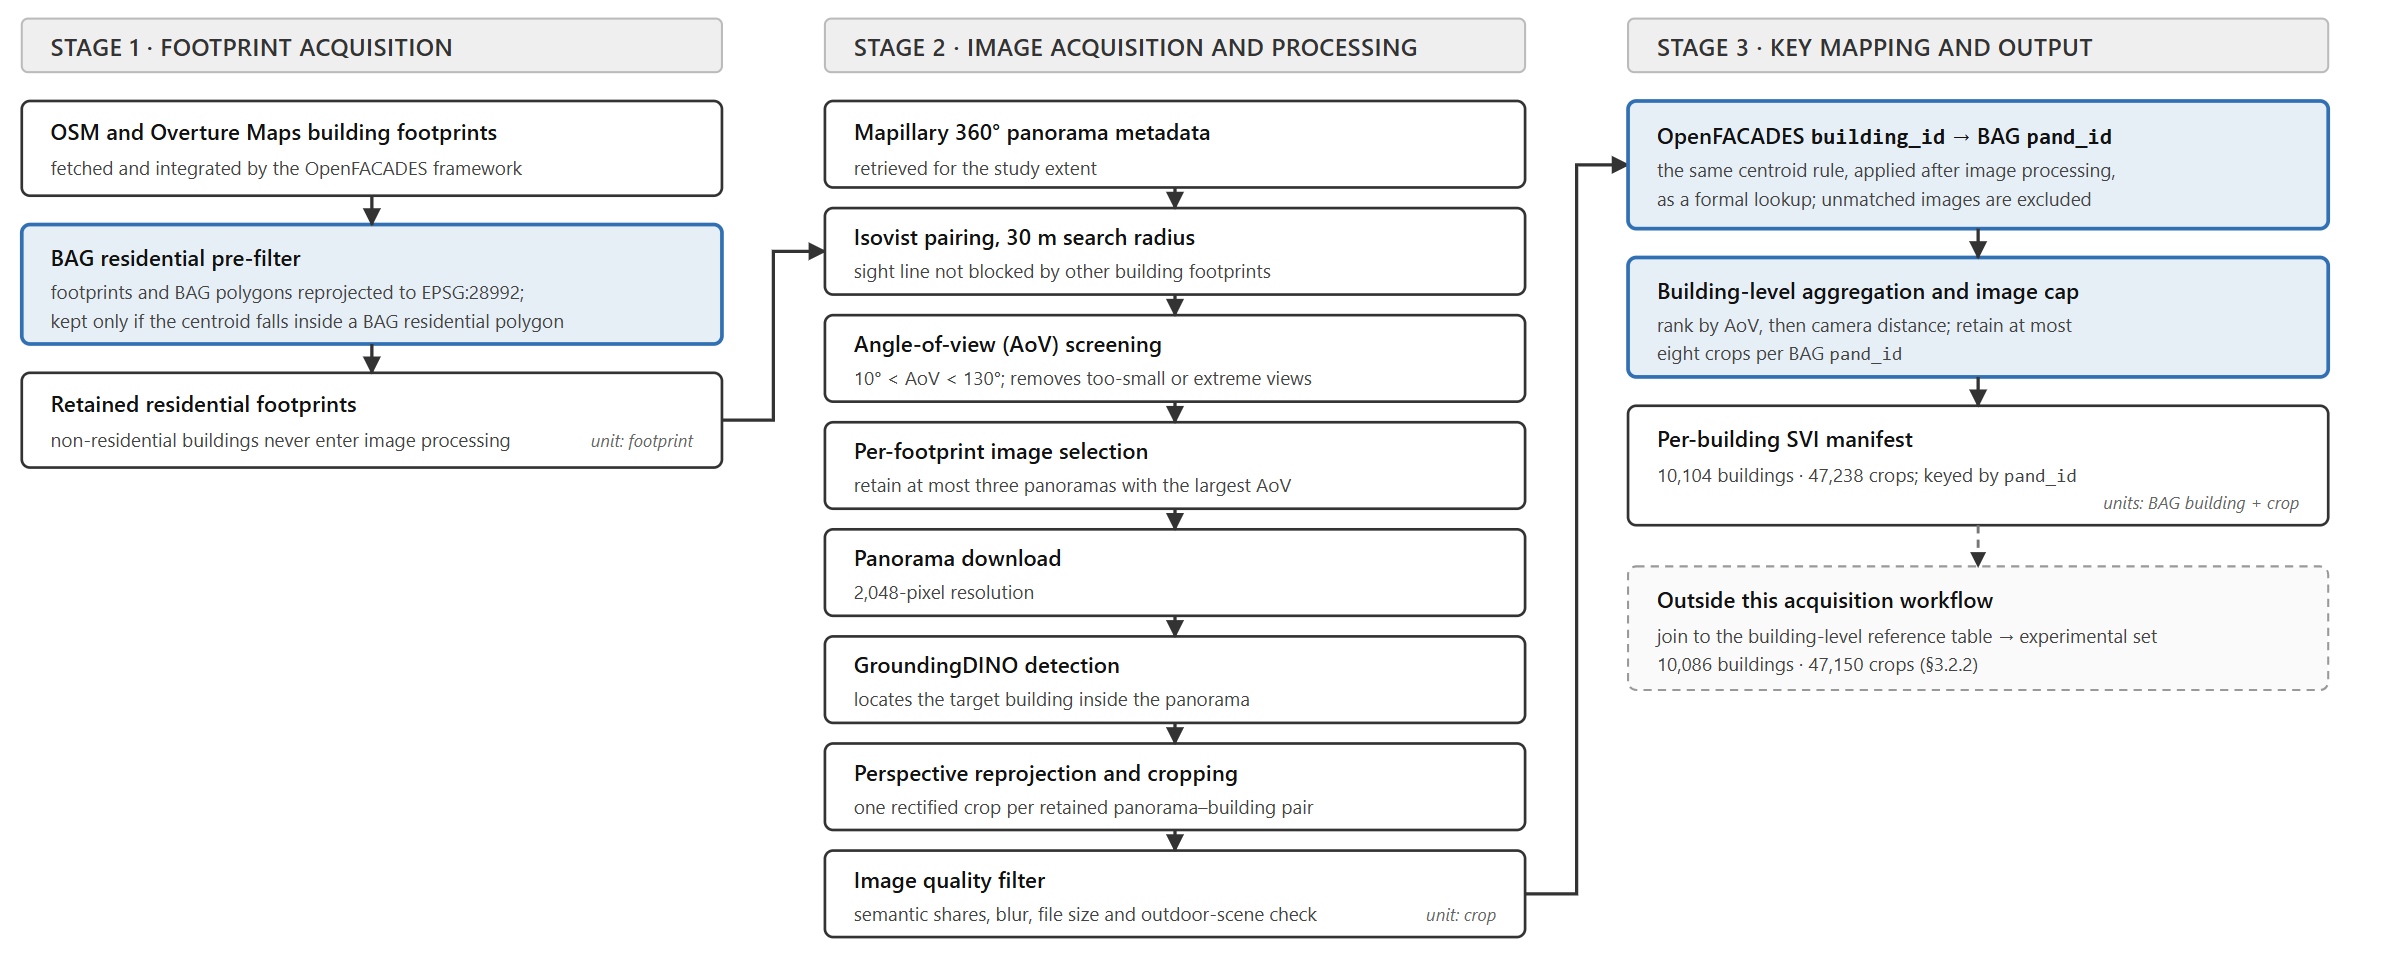
\includegraphics[width=0.98\linewidth,height=0.78\textheight,keepaspectratio]{figures/fig/fig_3_3_svi_workflow.png}
\caption{SVI acquisition and processing workflow.}
\label{fig:3_3}
\end{figure}

\begin{figure}[htbp]
\centering
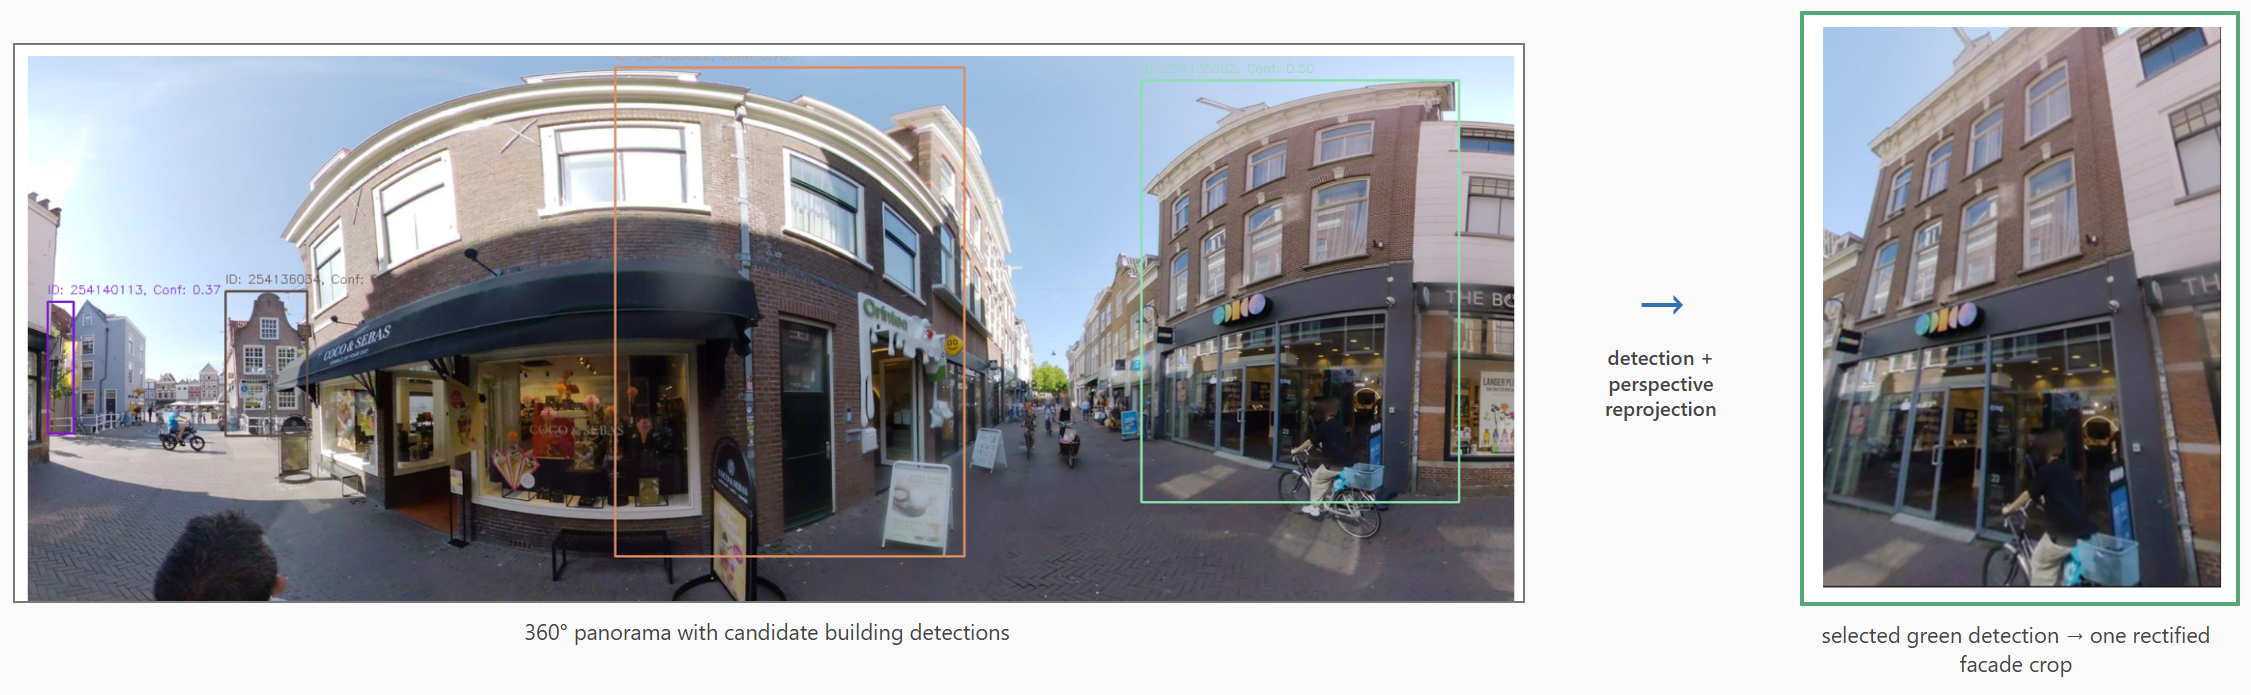
\includegraphics[width=0.98\linewidth,height=0.38\textheight,keepaspectratio]{figures/fig/fig_3_3_detail.png}
\caption*{Panorama detection and facade-crop reprojection.}
\end{figure}


\textbf{Building-level reference table and data linkage.} The building reference data and SVI manifest are constructed separately. The EP-Online data are first restricted to residential categories and existing-building certificates; where multiple records share the same BAG building identifier, only the record with the most recent registration date is retained. BAG, 3DBAG, and EP-Online are then joined using an inner join on \texttt{pand\_id}, after which TABULA-NL archetype lookup is performed based on building type and construction period to form the building-level reference table. Finally, the SVI manifest and the TABULA-matched reference table are joined using an inner join on \texttt{pand\_id}. The label uncertainty introduced by building-level aggregation based on the most recent certificate is examined further in \cref{sec:4_3_4}.


Records are selected and quality-controlled according to the following rules:


\begin{enumerate}
\item \textbf{Residential and existing buildings:} The BAG usage designation must include \texttt{woonfunctie}. EP-Online records must belong to the residential category (\texttt{Gebouwklasse = W}), have existing-building status (\texttt{Status = Bestaand}), and contain a non-missing \texttt{Energieklasse}. These conditions restrict the study scope to residential buildings and ensure compatibility with the TABULA-NL residential typology.
\item \textbf{Reference attributes and archetype matching:} Only buildings with \texttt{1800 <= bouwjaar <= 2025} are retained, thereby excluding missing, anomalous, or out-of-period construction years. The EP-Online \texttt{Gebouwtype} must map to one of the four residential types used in this study, the estimated floor count must lie between 1 and 30, and the building must permit TABULA-NL archetype matching.
\item \textbf{EPC record selection and methodological period:} When the same \texttt{BAGPandIDs} value is associated with multiple EP-Online certificates, the record with the most recent \texttt{Registratiedatum} is retained. The study does not explicitly filter for NTA 8800 certificates using \texttt{Berekeningstype}. However, in the EP-Online snapshot dated 1 April 2026, all certificates retained in the final sample were registered after 2021 and therefore fall within the period in which NTA 8800 was in effect.
\item \textbf{Geometric image--building pairing:} The Mapillary camera position must fall within a 30 m search radius of the target building, and an unobstructed geometric line of sight must exist between the camera and the building without intersection by another building footprint. Candidate pairings must also satisfy \texttt{10 deg < AoV < 130 deg} to exclude images in which the building is too small or the viewing angle is excessively oblique. This geometric assessment does not account for trees, vehicles, or other temporary obstructions.
\item \textbf{Image-quality filtering (heuristic):} A cropped image must satisfy all of the following conditions: a pixel proportion of at least 15\% for the \texttt{Building} class, a pixel proportion of no more than 30\% for the \texttt{Wall} class, Laplacian variance greater than 30, a file size of at least 20,000 bytes (approximately 20 kB), and an outdoor scene classification from Places365. These thresholds exclude images with targets that are too small, unsuitable visual content, severe blur, or anomalous files.
\item \textbf{Maximum image count:} Image counts are limited at two levels. During OpenFACADES image selection, a maximum of three panoramic images with the largest AoV values is retained for each OpenFACADES footprint. Because multiple OpenFACADES footprints may correspond to the same BAG \texttt{pand\_id}, a BAG building may still have more than three cropped images after identifier linkage. Images associated with the same \texttt{pand\_id} are therefore sorted by decreasing AoV and, where AoV values are equal, by increasing camera-to-building distance. A maximum of eight images is ultimately retained for each BAG building.
\end{enumerate}


The inclusion and exclusion rules and their corresponding sample counts are summarised in \cref{tab:3_2}. Because the workflow contains several distinct counting units, including OpenFACADES footprints, panorama--footprint pairs, cropped images, and BAG buildings, \cref{tab:3_2} reports the building and image counts separately at each stage rather than combining different units into a single funnel count.


After image-quality filtering, \texttt{pand\_id} linkage, and application of the eight-image-per-building limit, the SVI manifest contains \textbf{10,104 buildings and 47,238 images}. When the manifest is linked to the building-level reference table, 88 images associated with 18 buildings are excluded from the experimental dataset because of invalid 3DBAG geometry or unsuccessful TABULA-NL archetype matching. The final experimental dataset therefore contains \textbf{10,086 buildings and 47,150 images}.


The Mapillary image-acquisition dates and EPC registration dates are not temporally matched or filtered in this study. The potential temporal mismatch between images and labels is discussed in \cref{sec:5_2}. Representative cropped street-view images are shown in \cref{fig:3_4}.


\begin{table}[htbp]
\centering
\fbox{\begin{minipage}{0.88\textwidth}\centering
\textbf{Table placeholder}\\[0.6em]
Data inclusion and exclusion rules. The table reports the processing stage, counting unit, operational condition, design rationale, remaining building count, and remaining image count
\end{minipage}}
\caption{Data inclusion and exclusion rules. The table reports the processing stage, counting unit, operational condition, design rationale, remaining building count, and remaining image count}
\label{tab:3_2}
\end{table}


\begin{figure}[htbp]
\centering
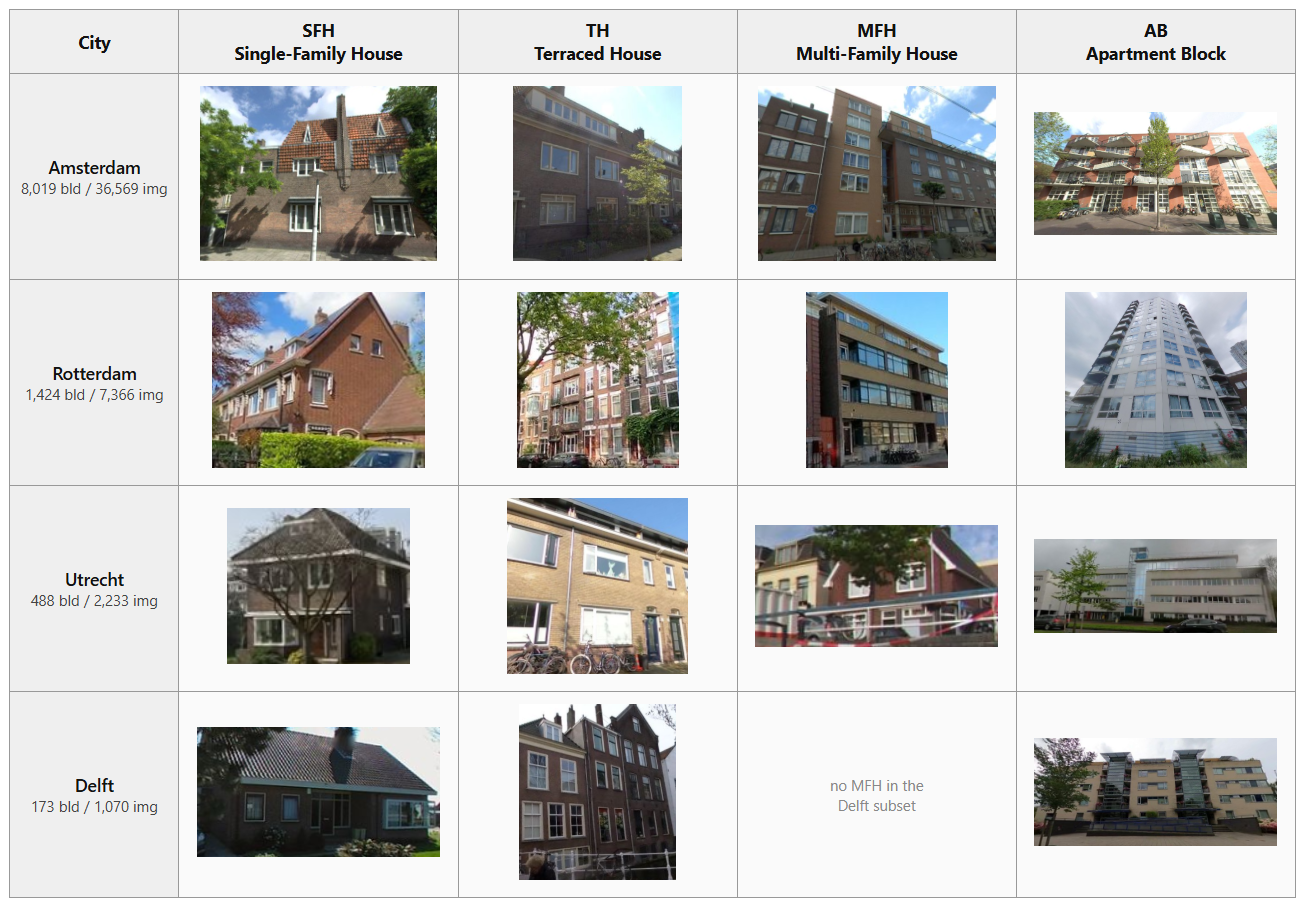
\includegraphics[width=0.98\linewidth,height=0.70\textheight,keepaspectratio]{figures/fig/fig_3_4_examples.png}
\caption{Representative street-view crops by city and size class.}
\label{fig:3_4}
\end{figure}


\subsection{Data Partitioning and Cross-Validation}
\label{sec:3_2_3}


The final experimental dataset is partitioned in two stages at the building level. In the first stage, five-fold \texttt{StratifiedGroupKFold} is applied to the 10,086 buildings, with one fold retained as a 20\% hold-out set comprising 2,018 buildings and the remaining 80\% used as a development set comprising 8,068 buildings. The stratification variable combines the study area (\texttt{city}), the original EP-Online residential-type field (\texttt{Gebouwtype}), the registered EP-Online energy-class field (\texttt{Energieklasse}), and the derived TABULA construction period (\texttt{tabula\_period}). BAG \texttt{pand\_id} is used as the grouping key to ensure that multiple images of the same building cannot be distributed across different data subsets.


In the second stage, five-fold cross-validation is performed within the development set using \texttt{StratifiedGroupKFold} again. For every trainable model, model fitting, hyperparameter selection, and model selection use only the development set. The frozen hold-out set does not participate in model selection and is used only for final evaluation. All comparison routes use the same data partition to ensure direct comparability of the model results.


\section{Vision Inference Strategies and Training Configurations}
\label{sec:3_3}


Three open-source vision-model configurations are specified in advance to represent full-model fine-tuning, supervised prediction-head training on a frozen self-supervised backbone, and vision-language model inference without parameter updating. The configurations differ simultaneously in model architecture, pre-training method, parameter-update scope, number of images used per building, and multi-image aggregation. The study therefore compares three complete and reproducible inference configurations rather than using a factorial experiment to isolate the causal effect of any individual training strategy. Closed-source commercial models are excluded because their model versions, access conditions, and long-term reproducibility are more difficult to control.



\begin{landscape}
\begin{table}[p]
\centering
\caption{Vision configurations used for building-attribute prediction}
\label{tab:3_3}
\small
\begin{tblr}{
  width = \linewidth,
  colspec = {X[1.7,l] X[1,l] X[1,l] X[1,l] X[1,r] X[1,l]},
  row{1} = {font=\bfseries},
  rowsep = 3pt,
  colsep = 4pt
}
\toprule
Configuration & Pre-trained weights & Parameters updated on the development set & Development labels used & Images per building & Multi-image aggregation \\
\midrule
ResNet-50 full fine-tuning & ImageNet-pre-trained ResNet-50 & Backbone, shared MLP, and three attribute-output heads & Complete development labels & Up to 8 & Image features averaged before building-level prediction \\
Frozen DINOv2 ViT-B/14 & \texttt{vit\_base\_patch14\_dinov2.lvd142m} & Shared MLP and three attribute-output heads only; backbone frozen & Complete development labels & Up to 8 & Image features averaged before building-level prediction \\
InternVL3-2B without parameter updating & \texttt{OpenGVLab/}\allowbreak\texttt{InternVL3-2B} & None & Fixed, class-balanced subset of 200 development buildings used for prompt design & Up to 3 & Mode for building type; median for construction year and floor count \\
\bottomrule
\end{tblr}
\end{table}
\end{landscape}


\textbf{Supervised attribute prediction.} ResNet-50 and DINOv2 both use up to eight images per building, each resized to 224 \ensuremath{\times} 224 pixels. Each image is first transformed into a feature vector by the same backbone, and the resulting vectors are averaged arithmetically at the building level. The mean feature vector passes through a shared 256-dimensional MLP, after which three separate output heads predict \texttt{Gebouwtype}, construction year, and floor count. The attribute-training objective is


\[
\mathcal{L}_{\mathrm{attr}}
= \mathcal{L}_{\mathrm{CE,type}}
+ \mathcal{L}_{\mathrm{MSE,year}}
+ \mathcal{L}_{\mathrm{MSE,floor}}.
\]


Building type uses cross-entropy loss weighted inversely by class frequency in the corresponding development training fold. Construction year and floor count are first normalised using the mean and standard deviation of that training fold, after which mean squared error is calculated. The three loss terms are summed with equal weights, which are not adjusted using hold-out data. ResNet-50 updates all parameters in the backbone, shared MLP, and three output heads; DINOv2 freezes the backbone and updates only the shared MLP and output heads. Both configurations are trained in five folds within the development set. Early stopping in each fold is based on the validation \texttt{Gebouwtype} macro-F1, and final hold-out evaluation uses the fold checkpoint with the highest development-validation \texttt{Gebouwtype} macro-F1.


\textbf{VLM-based attribute inference.} InternVL3-2B does not update model parameters using the study data. Instead, deterministic decoding returns JSON containing \texttt{building\_type}, \texttt{construction\_year}, and \texttt{num\_floors}. The prompt wording and output rules are designed using a fixed, class-balanced subset of 200 development buildings and then frozen before hold-out evaluation. Accordingly, ``zero-shot'' in this study means only that the model parameters are not trained or fine-tuned using the study data; it does not mean that the overall analytical workflow makes no use of development labels. Up to the first three ranked images are used for each building. Parseable image-level responses are aggregated at the building level: building type is determined by the mode, construction year by the median, and floor count by the rounded median. Responses that cannot be parsed or fall outside the permitted ranges are marked as invalid and excluded from aggregation.


\textbf{Direct EPC prediction (M2).} In addition to the building-attribute models used for the M3 route, direct energy-label prediction configurations are established for the M2 route. For ResNet-50 and DINOv2, the three attribute-output heads are replaced by a single energy-classification head. The seven-class \texttt{Energieklasse} task and the binary A--C/D--G task are trained independently using cross-entropy loss weighted inversely by class frequency in the corresponding development training fold. ResNet-50 undergoes full-model fine-tuning for M2. DINOv2 instead uses pre-extracted and cached building-level mean features and trains only the energy-classification network. Checkpoint selection within each fold and selection of the final fold are both based on development-validation energy-label macro-F1. InternVL3-2B uses separate direct-prediction prompts for the seven-class and binary tasks. Each image produces one class response, and the final prediction is obtained by majority voting at the building level.


Because the two supervised configurations use up to eight images with feature-level aggregation, whereas InternVL3-2B uses up to three images with prediction-level aggregation, their results should be interpreted as comparisons between complete model configurations. The independent effects of image count and aggregation method are outside the identification scope of this study.


\Cref{fig:3_5} summarises the input, parameter-update scope, multi-image aggregation, and prediction outputs of the three vision-inference configurations.


\begin{figure}[htbp]
\centering
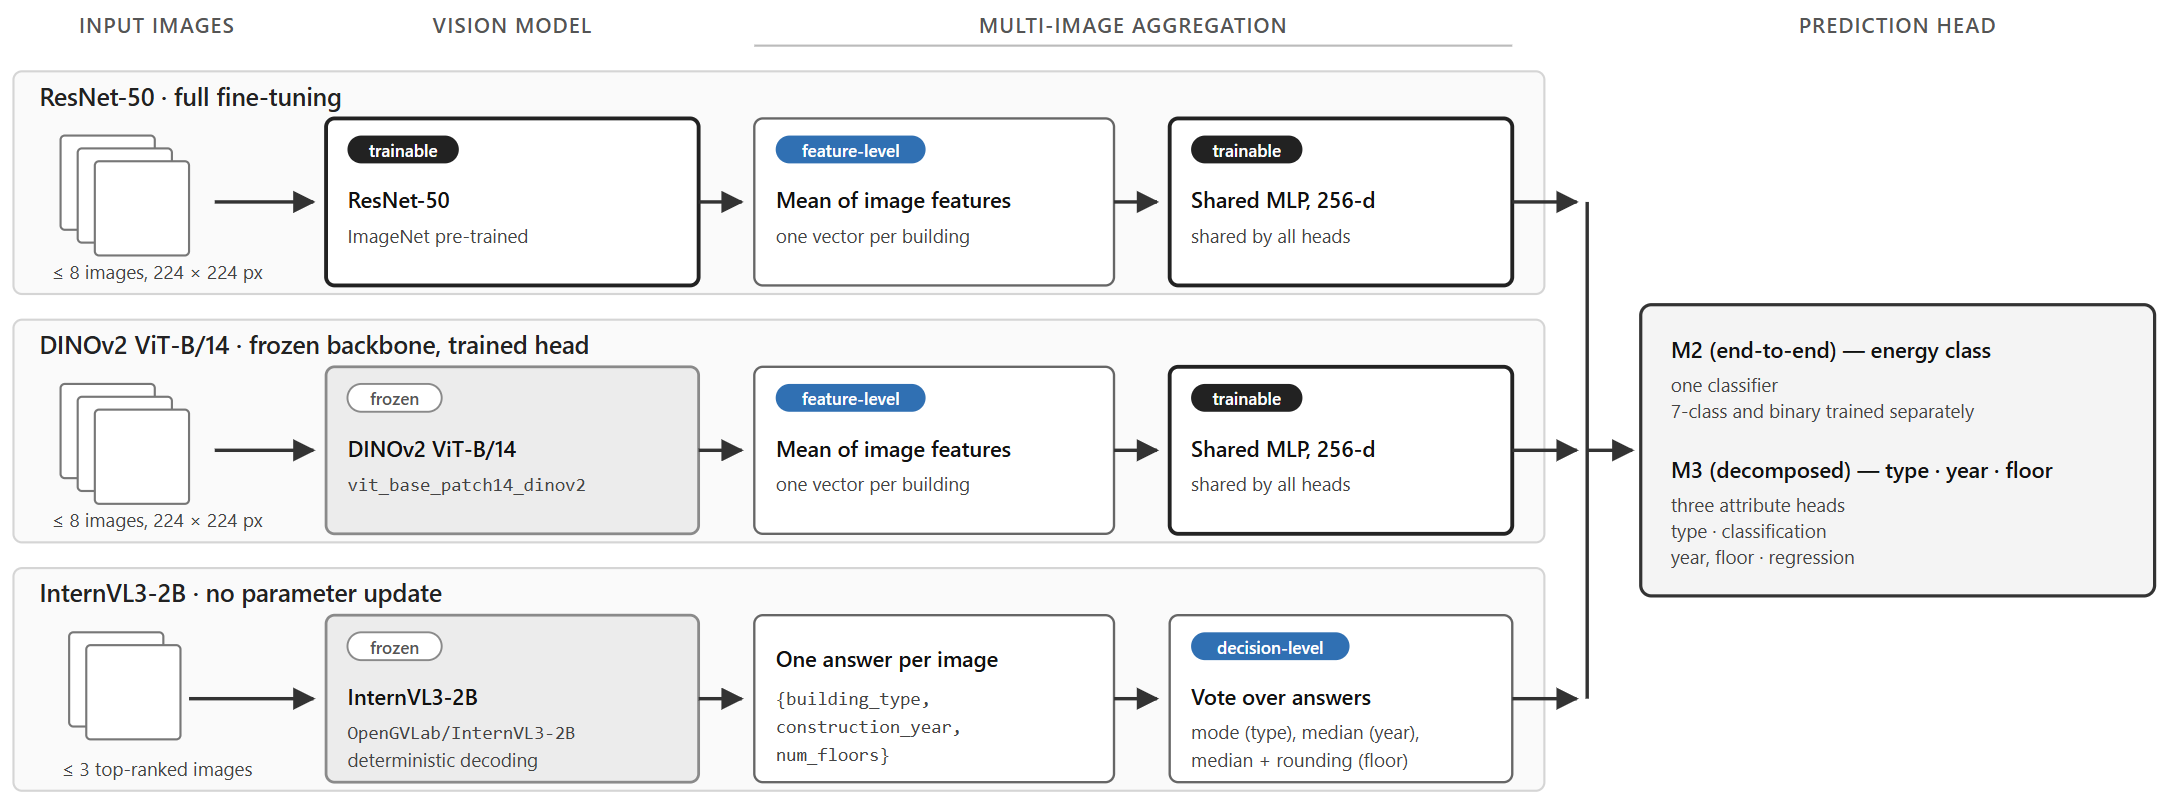
\includegraphics[width=0.98\linewidth,height=0.78\textheight,keepaspectratio]{figures/fig/fig_3_5_vision_models.png}
\caption{Vision-model configurations and multi-image aggregation.}
\label{fig:3_5}
\end{figure}


\section{TABULA Archetype Matching}
\label{sec:3_4}


\subsection{NL Matrix Structure}
\label{sec:3_4_1}


The Dutch TABULA matrix consists of six construction periods \ensuremath{\times} four size classes, forming 24 archetype cells in total (\cref{fig:3_6}). Each cell corresponds to a TABULA-NL archetype identifier that is subsequently used to retrieve the associated as-built thermal parameters. The period boundaries and operational definitions of the size classes are taken from the Dutch TABULA national typology report, the RVO \emph{Example Dwellings} (\emph{Voorbeeldwoningen}) series, rather than from \hyperlink{ref:loga2016}{Loga et al. (2016)}. The latter provides a methodological and cross-national comparison framework but does not contain the Dutch classification thresholds.


\begin{figure}[htbp]
\centering
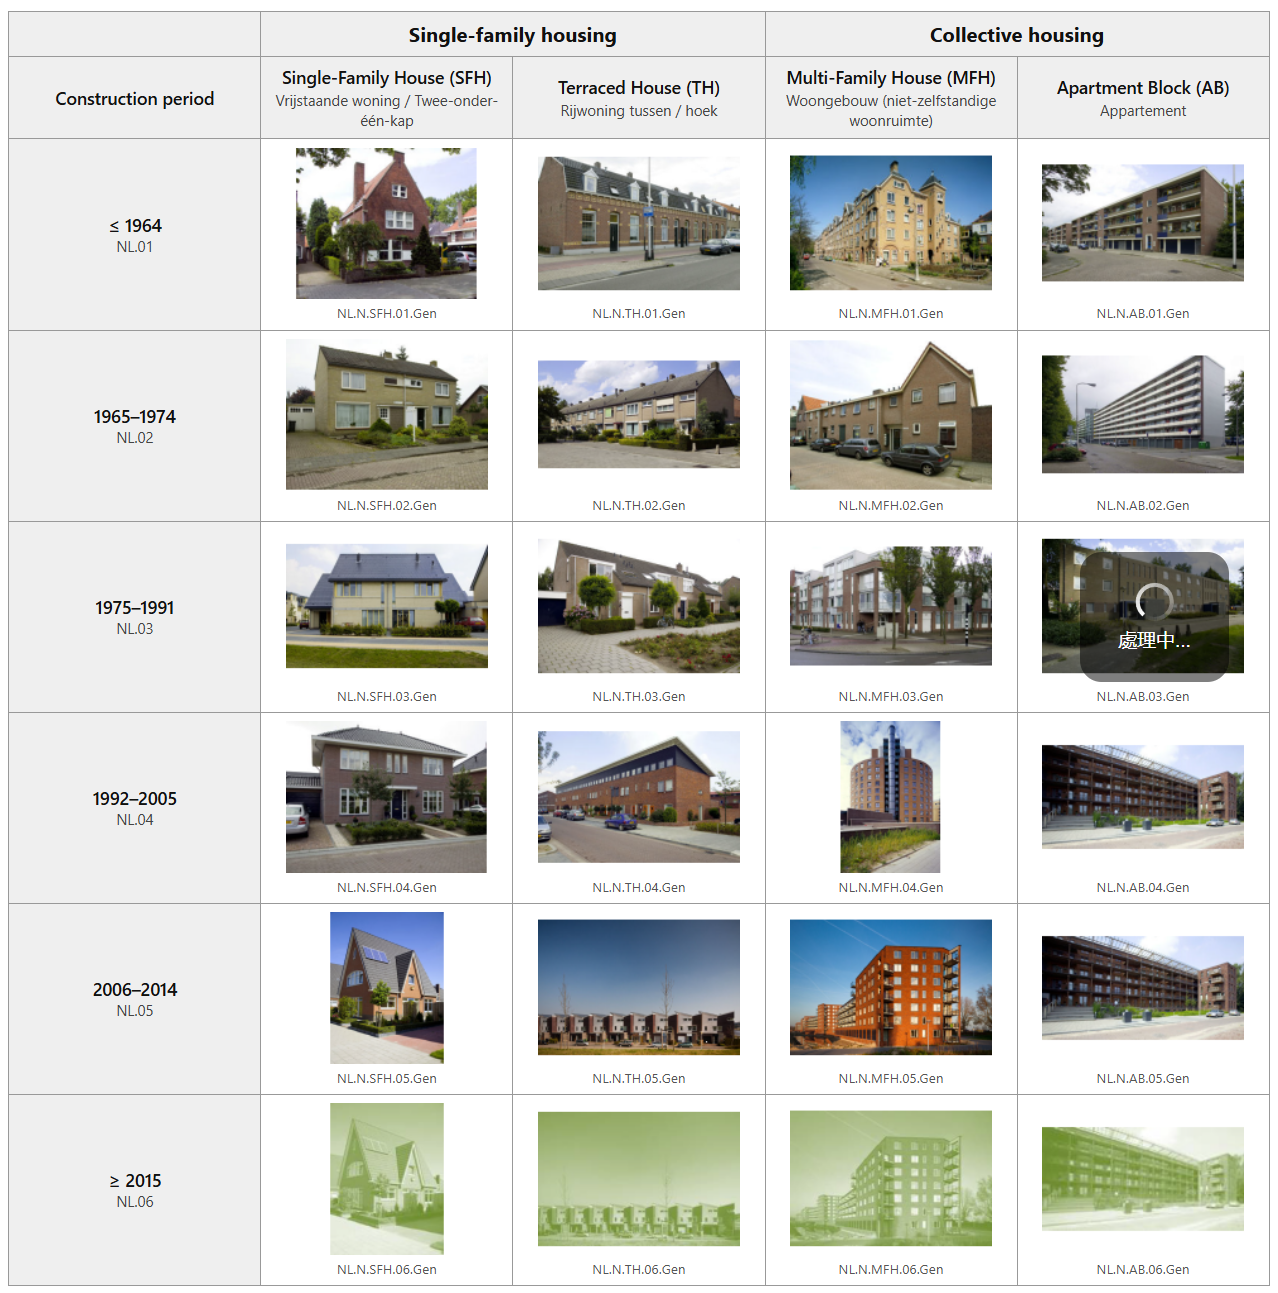
\includegraphics[width=0.98\linewidth,height=0.70\textheight,keepaspectratio]{figures/fig/fig_3_6_tabula_matrix.png}
\caption{TABULA-NL residential typology matrix.}
\label{fig:3_6}
\end{figure}


\textbf{Size-class definitions.} The four size classes are defined according to the Dutch dwelling types represented in the TABULA-NL matrix; no additional thresholds based on the number of dwelling units or floors are imposed:


\begin{itemize}
\item \textbf{SFH --- Single-Family House:} Detached house (\texttt{Vrijstaande woning}) and semi-detached house (\texttt{Twee-onder-één-kap}).
\item \textbf{TH --- Terraced House:} Mid-terrace house (\texttt{Rijwoning tussen}) and end-terrace house (\texttt{Rijwoning hoek}).
\item \textbf{MFH --- Multi-Family House:} Residential building with non-self-contained accommodation (\texttt{Woongebouw met niet-zelfstandige woonruimte}).
\item \textbf{AB --- Apartment Block:} Apartment (\texttt{Appartement}).
\end{itemize}


\subsection{Attribute-to-Archetype Mapping}
\label{sec:3_4_2}


The TABULA-NL archetype cell of each building is jointly determined by its building size class and construction period. Let \(s_i\) denote the TABULA size class of building \(i\), and let \(p(y_i)\) denote the construction period obtained by discretising construction year \(y_i\) according to the boundaries shown in \cref{fig:3_6}. The archetype cell is then defined as


\[
c_i = \bigl(s_i, p(y_i)\bigr).
\]


In the reference-attribute route, construction year is obtained from the BAG \texttt{bouwjaar}, while the EP-Online building type (\texttt{Gebouwtype}) is converted deterministically to SFH, TH, MFH, or AB according to \cref{tab:3_4}. In the vision-attribute route, the model predicts these four TABULA size classes directly and does not use the EP-Online \texttt{Gebouwtype} enumeration as an intermediate mapping. The predicted continuous construction year is discretised using the same period boundaries. Both routes use the same archetype lookup at this stage; they differ only in whether the input attributes originate from reference data or vision predictions.



\begin{table}[H]
\centering
\caption{Operational mapping from EP-Online building type (\texttt{Gebouwtype}) to TABULA-NL size class}
\label{tab:3_4}
\small
\begin{tblr}{
  width = \linewidth,
  colspec = {X[1,l] X[1,l]},
  row{1} = {font=\bfseries},
  rowsep = 3pt,
  colsep = 4pt
}
\toprule
EP-Online building type (\texttt{Gebouwtype}) & TABULA-NL size class \\
\midrule
Detached house (\texttt{Vrijstaande woning}) & SFH \\
Semi-detached house (\texttt{Twee-onder-één-kap}) & SFH \\
Mid-terrace house (\texttt{Rijwoning tussen}) & TH \\
End-terrace house (\texttt{Rijwoning hoek}) & TH \\
Residential building with non-self-contained accommodation (\texttt{Woongebouw met niet-zelfstandige woonruimte}) & MFH \\
Apartment (\texttt{Appartement}) & AB \\
\bottomrule
\end{tblr}
\end{table}


\Cref{tab:3_4} defines the deterministic operational mapping adopted in this study. The reference-attribute route maps the EP-Online enumeration values directly and does not reclassify building type from street-view imagery. Records outside the six retained values listed above are excluded during construction of the building-level reference dataset. All archetype assignments use BAG \texttt{pand\_id} as the unit of analysis and the retained EP-Online record defined in \cref{sec:3_2_2}; the resulting unit-of-observation limitation is discussed in \cref{sec:5_1_2}.


Floor count does not participate in archetype-cell assignment because the TABULA-NL lookup key consists only of size class and construction period. \texttt{num\_floors} is nevertheless retained as a separate feature in the downstream EPC-classification model.


\subsection{U-Value Lookup and As-Built Assumption}
\label{sec:3_4_3}


After archetype-cell assignment, the wall, roof, floor, and window U-values are retrieved from the TABULA-NL lookup table according to the building's size class and construction period. All four values are expressed in \(W/(m^2K)\). The reference-attribute route performs the lookup using the reference building type and construction year, while the vision-attribute route applies the same procedure using the image-inferred building type and construction year. The U-values, element variants, and source records for each cell are provided in Appendix A.


Because renovation status is unavailable at the individual-building level, every building is assigned the unrenovated existing-state, or as-built, variant of its TABULA-NL cell. This is a modelling assumption rather than an observation of the building's current envelope condition. For thermally renovated buildings, the assigned U-values may exceed the current actual thermal transmittance and may therefore overestimate transmission heat loss.


TABULA-NL U-values represent archetype-level assumptions for the corresponding building-stock subgroup rather than measured thermal parameters for individual buildings \hyperlink{ref:loga2016}{(Loga et al., 2016)}. Buildings with the same size class and construction period therefore receive the same four U-values; these values cannot establish the actual envelope construction or renovation status of an individual building.


\section{Downstream EPC Classification Model}
\label{sec:3_5}


A LightGBM gradient-boosting classifier \hyperlink{ref:ke2017}{(Ke et al., 2017)} is used as the downstream EPC-classification model. LightGBM is suitable for low-dimensional tabular data comprising numerical and categorical variables and allows the same model architecture and training configuration to be maintained across different attribute sources. In this study, it serves as a controlled downstream evaluator for quantifying the effect of replacing reference attributes with image-inferred attributes on EPC prediction; it is not presented as a contribution of a new classification algorithm.


The model has eight core input fields: building type, construction year, floor count, wall U-value, roof U-value, floor U-value, window U-value, and city. Building type and city are treated as categorical features, while the remaining fields are numerical features. The reference-attribute route uses the reference building type, construction year, and floor count and obtains the four U-values from the corresponding TABULA-NL cell. The vision-attribute route instead uses the three image-inferred attributes and retrieves the U-values from the predicted TABULA-NL cell. The two routes therefore have the same eight-field feature schema, and city remains unchanged; the only differences arise from the source of the three upstream attributes and their derived archetype U-values. Apart from the EPC target label and the fields used to construct the reference attributes, no other certificate-derived variables are used because they would be unavailable for target buildings without an existing energy certificate.


The seven-class A--G and binary A--C/D--G EPC tasks use two independently trained LightGBM classifiers with multiclass and binary objectives, respectively. Both tasks use the same fixed hyperparameter configuration, without route-specific tuning. The principal settings are 400 boosting iterations, a learning rate of 0.05, 31 leaves, and no class weighting; the complete configuration is provided in Appendix A.


The final downstream classifier is fitted once on the complete development set using reference features. The same fitted model is then applied separately to the reference-derived and vision-derived hold-out features. This protocol avoids introducing additional differences through downstream-model retraining, so that the prediction gap reflects the combined consequences of attribute substitution and propagation through the TABULA lookup. The development evaluation, hold-out protocol, and evaluation metrics are described in \cref{sec:4_1}.
